\chapter{Escenario de Pruebas}

El escenario de pruebas seleccionado para la evaluación de nuestro protocolo es el campo deportivo de la UPIITA-UPIBI del IPN, ubicado en La Laguna Ticomán, Gustavo A. Madero, Ciudad de México. Este espacio es un área verde con acceso exclusivo para estudiantes, profesores y personal del IPN. Para la realización de las pruebas, se instalará una red de sensores inalámbricos (WSN) en una zona del campo. Los sensores recopilarán datos relacionados con variables ambientales como la temperatura, y datos de los animales como las coordenadas GPS y el video de las cámaras trampa. Estos datos permitirán monitorear el entorno y obtener información relevante para la evaluación del sistema.\\
Para obtener resultados más realistas y representativos, se simulará el comportamiento de una especie animal específica dentro del escenario de pruebas. Se utilizarán modelos de simulación basados en el conocimiento existente sobre la especie, su comportamiento y sus interacciones con el entorno. Estos modelos permitirán generar datos simulados que representen los patrones de movimiento, las interacciones y las preferencias de hábitat de la especie en cuestión.\\
Posteriormente, se desplegará un enjambre de drones para recolectar los datos de monitoreo de la WSN. Durante el despliegue, los drones operarán bajo la coordinación del protocolo propuesto, el cual permitirá un mejor control de los drones y asegurará la eficiencia en la recolección de datos.\\
Además, se llevarán a cabo pruebas para evaluar la eficacia de la recolección de datos durante diferentes momentos del día y bajo diferentes condiciones climáticas, para simular posibles condiciones y evaluar el desempeño del sistema en diferentes escenarios. Durante estas pruebas, se medirán parámetros de desempeño específicos para evaluar el funcionamiento del sistema.\\
Para medir y cuantificar los resultados de cada parámetro de desempeño, se utilizarán métricas específicas. Estas métricas podrían incluir el porcentaje de datos recopilados correctamente, la tasa de errores en la transmisión de datos y el tiempo promedio de respuesta. Las mediciones se llevarán a cabo siguiendo procedimientos establecidos, utilizando herramientas o software especializados y aplicando protocolos de medición adecuados.\\
Con esta selección, se busca simular un escenario que permita evaluar la eficacia del sistema en situaciones de alta demanda y diferentes condiciones ambientales. De igual manera, se va a utilizar software de simulación para el vuelo de los drones, y se van a desarrollar algunas simulaciones para la red de sensores. Las pruebas se realizarán en cada una de las siguientes tres etapas:

\begin{enumerate}
    \item Pruebas preliminares de vuelo del subsistema de enjambre.
\end{enumerate}
    \newpage
\begin{figure}[H]
    \centering
    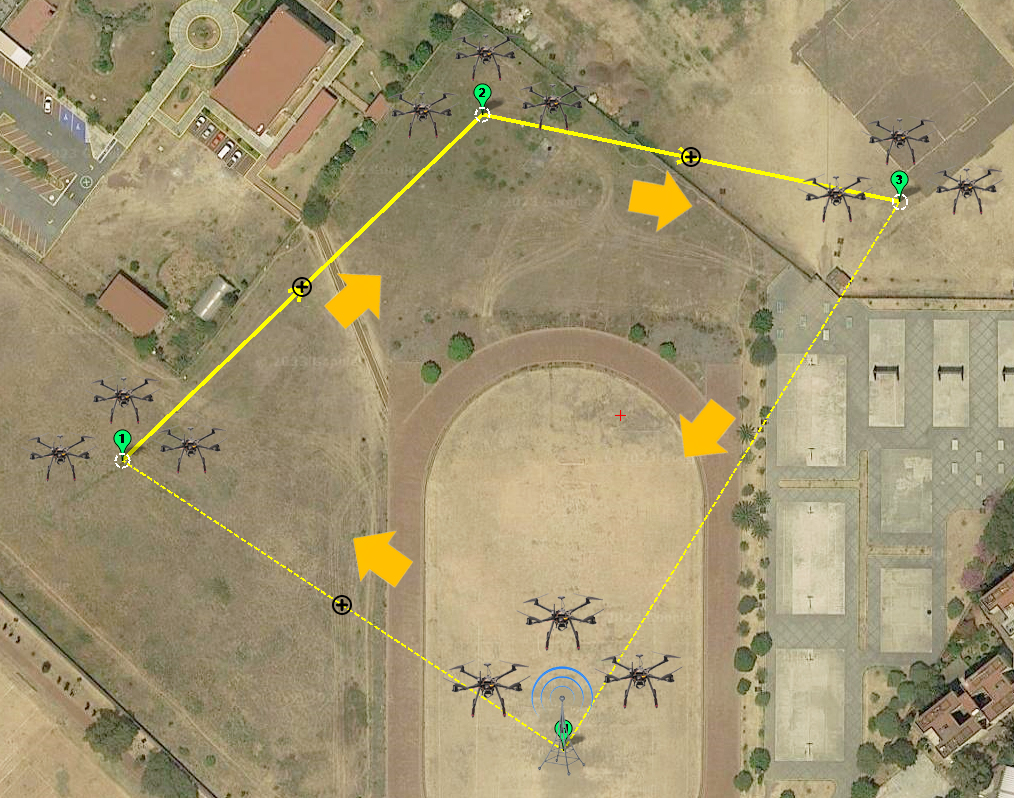
\includegraphics[width=0.6\linewidth]{imagenes/1_1.jpg}
    \caption{Escenario de pruebas finales del subsistema enjambre en el campo UPIITA-UPIBI.}
    \label{fig:enter-label}
\end{figure}

\begin{enumerate}[start=2]
    \item Pruebas preliminares de comunicación del subsistema de la WSN.
\end{enumerate}

\begin{figure}[H]
    \centering
    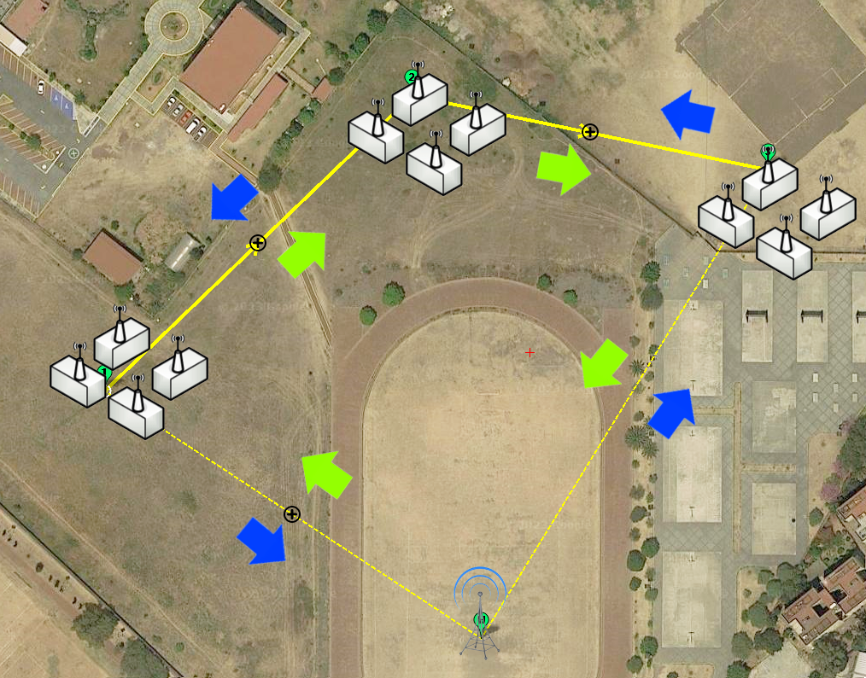
\includegraphics[width=0.65\linewidth]{imagenes/2.png}
    \caption{Escenario de pruebas finales del subsistema WSN en el campo UPIITA-UPIBI.}
    \label{fig:enter-label}
\end{figure}
\begin{enumerate}[start=3]
    \item Pruebas finales del sistema integrado.
\end{enumerate}

\begin{figure}[H]
    \centering
    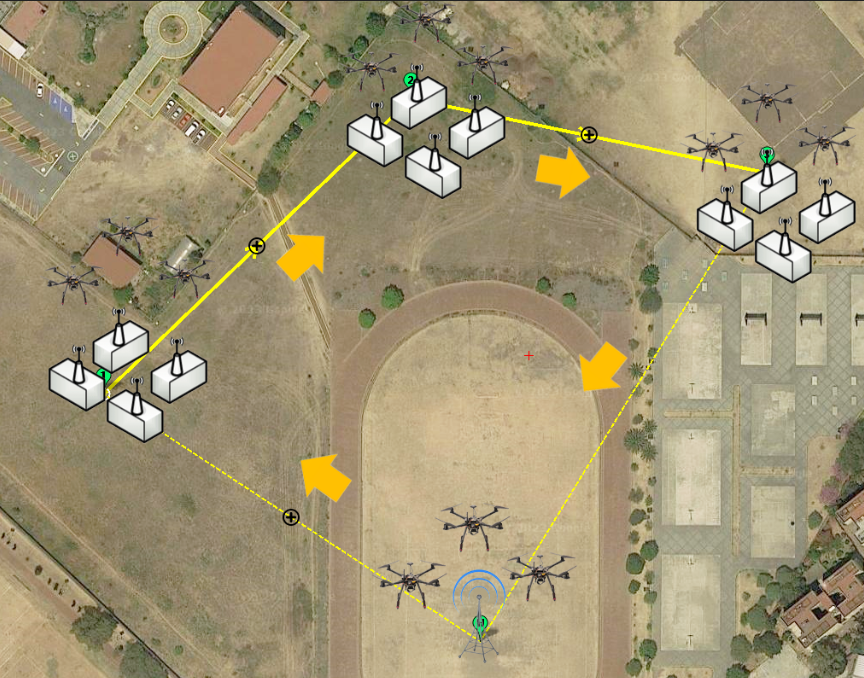
\includegraphics[width=0.75\linewidth]{imagenes/3.png}
    \caption{Escenario de pruebas finales del sistema integral en el campo UPIITA-UPIBI.}
    \label{fig:enter-label}
\end{figure}